\subsection{RANSAC-Based Motion Filtering}

A critical step in radar-based odometry is the separation of static landmarks from dynamic objects. 
This distinction ensures that ego-motion is estimated using only consistent reference points. 
To achieve this, a RANSAC-based filtering method is applied to the relationship between azimuth angle $\theta$ and Doppler velocity $v_d$.

\subsubsection*{Principle}
When the radar is mounted on a moving platform, static objects do not appear motionless. 
Instead, they exhibit Doppler velocities that depend on the vehicle’s own speed and the azimuth angle of detection. 
This results in a predictable curve when Doppler velocity is plotted against azimuth. 
Dynamic objects (e.g., moving vehicles or pedestrians) deviate from this pattern.  

RANSAC (Random Sample Consensus) is used to robustly fit a polynomial model to the Doppler–azimuth distribution of static points. 
Inliers to the model are considered static reflections, while outliers are classified as dynamic.

\subsubsection*{Mathematical Model}
The relationship between azimuth angle and Doppler velocity is modeled as a quadratic function:
\[
v_d = a\theta^2 + b\theta + c.
\]

Let $\mathbf{X}$ be the azimuth vector and $\mathbf{y}$ the Doppler velocities:
\[
\mathbf{X} = \begin{bmatrix} \theta_1 \\ \theta_2 \\ \vdots \\ \theta_n \end{bmatrix}, \quad 
\mathbf{y} = \begin{bmatrix} v_{d1} \\ v_{d2} \\ \vdots \\ v_{dn} \end{bmatrix}.
\]

RANSAC estimates the coefficients $\mathbf{w} = [a, b, c]^T$ by iteratively:
\begin{itemize}
    \item Sampling minimal subsets of $(\theta, v_d)$ pairs,
    \item Fitting the polynomial model,
    \item Counting inliers with residual error below a threshold,
    \item Selecting the model with the largest consensus set.
\end{itemize}

This approach is robust to noisy points and moving targets that would otherwise distort the fit.

\subsubsection*{Integration into the Pipeline}
The RANSAC-based motion filter is applied after coordinate and Doppler thresholding. 
It outputs:
\begin{itemize}
    \item \textbf{Inliers} - points likely to be static, used for clustering and ICP alignment,
    \item \textbf{Outliers} - points likely dynamic, excluded from ego-motion estimation.
\end{itemize}

\begin{figure}[!htbp]
    \centering
    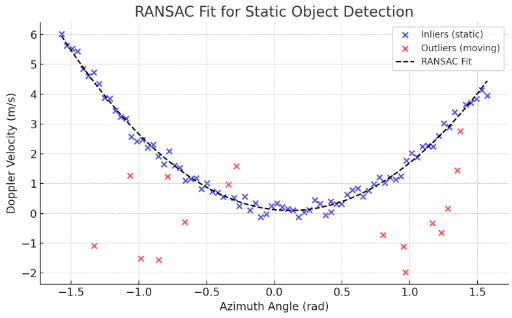
\includegraphics[width=1.0\linewidth]{images/RANSAC.png}
    \caption{RANSAC fit of Doppler vs. azimuth. Inliers = static (blue), Outliers = moving (red).\\
    \textit{Note: This figure uses simulated data to illustrate the concept.}}
    \label{fig:ransac_simulated_static_dynamic}
\end{figure}

\begin{figure}[!htbp]
    \centering
    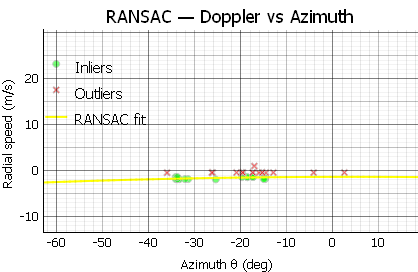
\includegraphics[width=1.0\linewidth]{images/RANSAC_movingTarget_wPtCloud.png}
    \caption{RANSAC fit of Doppler vs. azimuth. Inliers = static (green), Outliers = moving (red).\\
    \textit{Note: This figure shows real data when the vehicle is moving and a dynamic target is present.}}
    \label{fig:ransac_real_static_dynamic}
\end{figure}

\begin{figure}[!htbp]
    \centering
    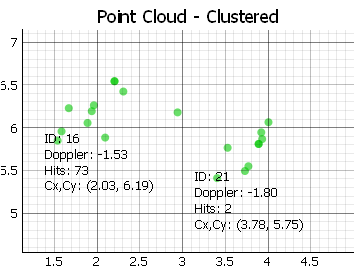
\includegraphics[width=1.0\linewidth]{images/RANSAC_movingTarget_ptCloud.png}
    \caption{Clustered point cloud corresponding to the RANSAC analysis in Fig.~\ref{fig:ransac_real_static_dynamic}. 
    Each cluster is annotated with ID, Doppler average, and centroid coordinates.}
    \label{fig:ransac_clustered_ptcloud}
\end{figure}

\begin{figure}[!htbp]
    \centering
    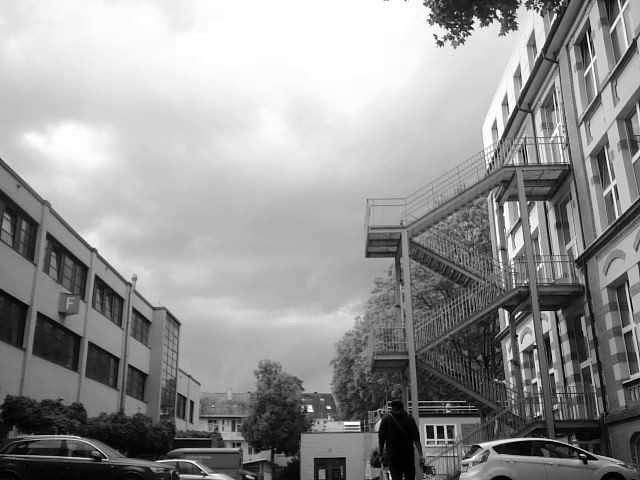
\includegraphics[width=1.0\linewidth]{images/frame_15s.png}
    \caption{Video frame at $t=15$ seconds, showing the target in the scene. 
    This frame corresponds to the radar data used in Figs.~\ref{fig:ransac_real_static_dynamic} and \ref{fig:ransac_clustered_ptcloud}.}
    \label{fig:frame_15s_target}
\end{figure}

\subsubsection*{Role of Doppler in Static vs. Dynamic Separation}
For a vehicle moving at velocity $v_e$, static reflections follow a Doppler distribution determined by the projection of $v_e$ along the radar line of sight. 
For example:
\begin{itemize}
    \item A static object directly in front exhibits $v_d \approx v_e$,
    \item A static object at $90^\circ$ azimuth exhibits $v_d \approx 0$,
    \item Intermediate azimuths follow a smooth transition between these extremes.
\end{itemize}

Dynamic objects violate this pattern, appearing as outliers in the Doppler-azimuth plane. 
This behavior is illustrated first on simulated data in Fig.~\ref{fig:ransac_simulated_static_dynamic}, and then validated on real measurements in Fig.~\ref{fig:ransac_real_static_dynamic}, where the presence of a moving target is evident.  
The corresponding clustered point cloud is shown in Fig.~\ref{fig:ransac_clustered_ptcloud}, where each object is assigned a unique identifier and centroid. Finally, the physical scene is provided in Fig.~\ref{fig:frame_15s_target}, which contextualizes the detected target in the real environment.

\vspace{1cm}
\paragraph*{Benefits of RANSAC-Based Filtering}
\begin{itemize}
    \item Robust against noise and measurement errors,
    \item Separates dynamic actors from static landmarks without prior labeling,
    \item Provides stable input for clustering and prevents moving objects from corrupting ego-motion estimation.
\end{itemize}

The output of this module is a refined point cloud in which only consistent static reflections contribute to downstream clustering and ICP alignment. 
In this system, RANSAC therefore plays a dual role: it filters out dynamic objects while simultaneously delivering a coherent static inlier set that underpins clustering stability and ICP-based odometry. 
As errors in static-dynamic separation would otherwise propagate downstream, this step is foundational for trajectory accuracy.


The integration of RANSAC-based motion filtering further ensures that odometry remains resilient in challenging scenarios, such as cluttered urban environments or mixed traffic conditions, where dynamic objects may dominate the scene. 
By anchoring estimation on reliable static structures, the system achieves greater robustness and consistency—critical factors for autonomous navigation. 
Additionally, maintaining a coherent model of the static Doppler pattern allows for a more accurate estimation of the vehicle's own self-speed, reinforcing the central role of RANSAC in radar-only odometry.
